\chapter{Desarrollo}
\section{Integración de prácticas de la cultura DevOPS al sistema de monitorio de ruido}
\subsection{Integración continua y despliegue continuo en el SMR}
Mitesh \cite {ci} define la Integración Continua (CI) como `` una práctica de desarrollo de software en la que los miembros de un equipo integran su trabajo con frecuencia '', también menciona uno de sus usos `` las organizaciones pueden realizar una integración continua de su código y verificar la integridad de el código en las primeras etapas de desarrollo ". La integración continua permite a los equipos integrar su trabajo y verificar (con pruebas unitarias) que todo está en condiciones óptimas antes de pasar al siguiente paso. La implementación continua (CD) también es una práctica de software que tiene lugar después de CI, los autores de \cite {CD} mencionan que ``el objetivo de la práctica de implementación continua es implementar de forma automática y constante todos los cambios en el entorno de producción ", en otras palabras poner cualquier cambio a disposición de los clientes.

Cada repositorio del Sistema NMS tiene dos ramas principales de git, Master y QA, la función de cada una es la siguiente:

\begin {itemize}
\item QA: esta es la rama principal para integrar todos los cambios en el código. Todo el código nuevo se prueba y analiza antes de poder enviarlo a esta rama.
\item Master: La rama de producción, donde el producto de software completa su último paso donde estará disponible para los consumidores.
\end {itemize}

\begin{figure}[H]
	\centering
	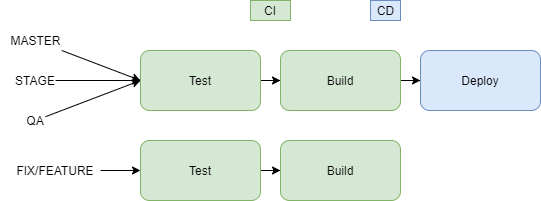
\includegraphics[width=\linewidth]{bibliografia/Imagenes/ci_cd branch Diagram.png}
	\caption{Diagrama de ramas y pipelines, el color indica que paso hace parte de la integración y el despliegue}
	\label{pipelines}
\end{figure}

Cada rama cuenta con  una serie de pasos como pueden observarse en la Figura \ref{pipelines} cuya función es la siguiente:
\begin{itemize}
\item Test: La aplicación de pruebas unitarias sobre todo el código para verificar la integridad del desarrollo y evitar que una funcionalidad pueda verse comprometida.
\item Build: El componente está preparado para ser implementado (crear una imagen, comprimir el código, construir el código, etc.).
\item Deploy: Despliega el componente en el entorno de desarrollo.
\end{itemize}
